%% This is an example first chapter.  You should put chapter/appendix that you
%% write into a separate file, and add a line \include{yourfilename} to
%% main.tex, where `yourfilename.tex' is the name of the chapter/appendix file.
%% You can process specific files by typing their names in at the 
%% \files=
%% prompt when you run the file main.tex through LaTeX.
\chapter{Introduction}
\section{Motivation}
Large organizations increasingly use virtualization to consolidate server
and desktop applications in data centers, reduce operating costs, simplify administrative
tasks and improve performance scalability. As a key 
enabling technology behind {\em Cloud Computing}, virtualization
is shaping how computers will be used in the future.

An important reason for the success of server virtualization 
is that it resolves the tension between typically conflicting
goals of high isolation and effective resource utilization.
Ideally, organizations would prefer to isolate each server
application by assigning it to a dedicated machine.
However, this approach entails inefficient resource allocation
because each application typically utilizes only a modest fraction of a 
machine's hardware.
With the development of virtualization technology, applications
can be assigned dedicated virtual machines (VMs),
while many such VMs can be hosted by the same physical
host for high resource utilization.

\begin{figure}[p]
  \centering
  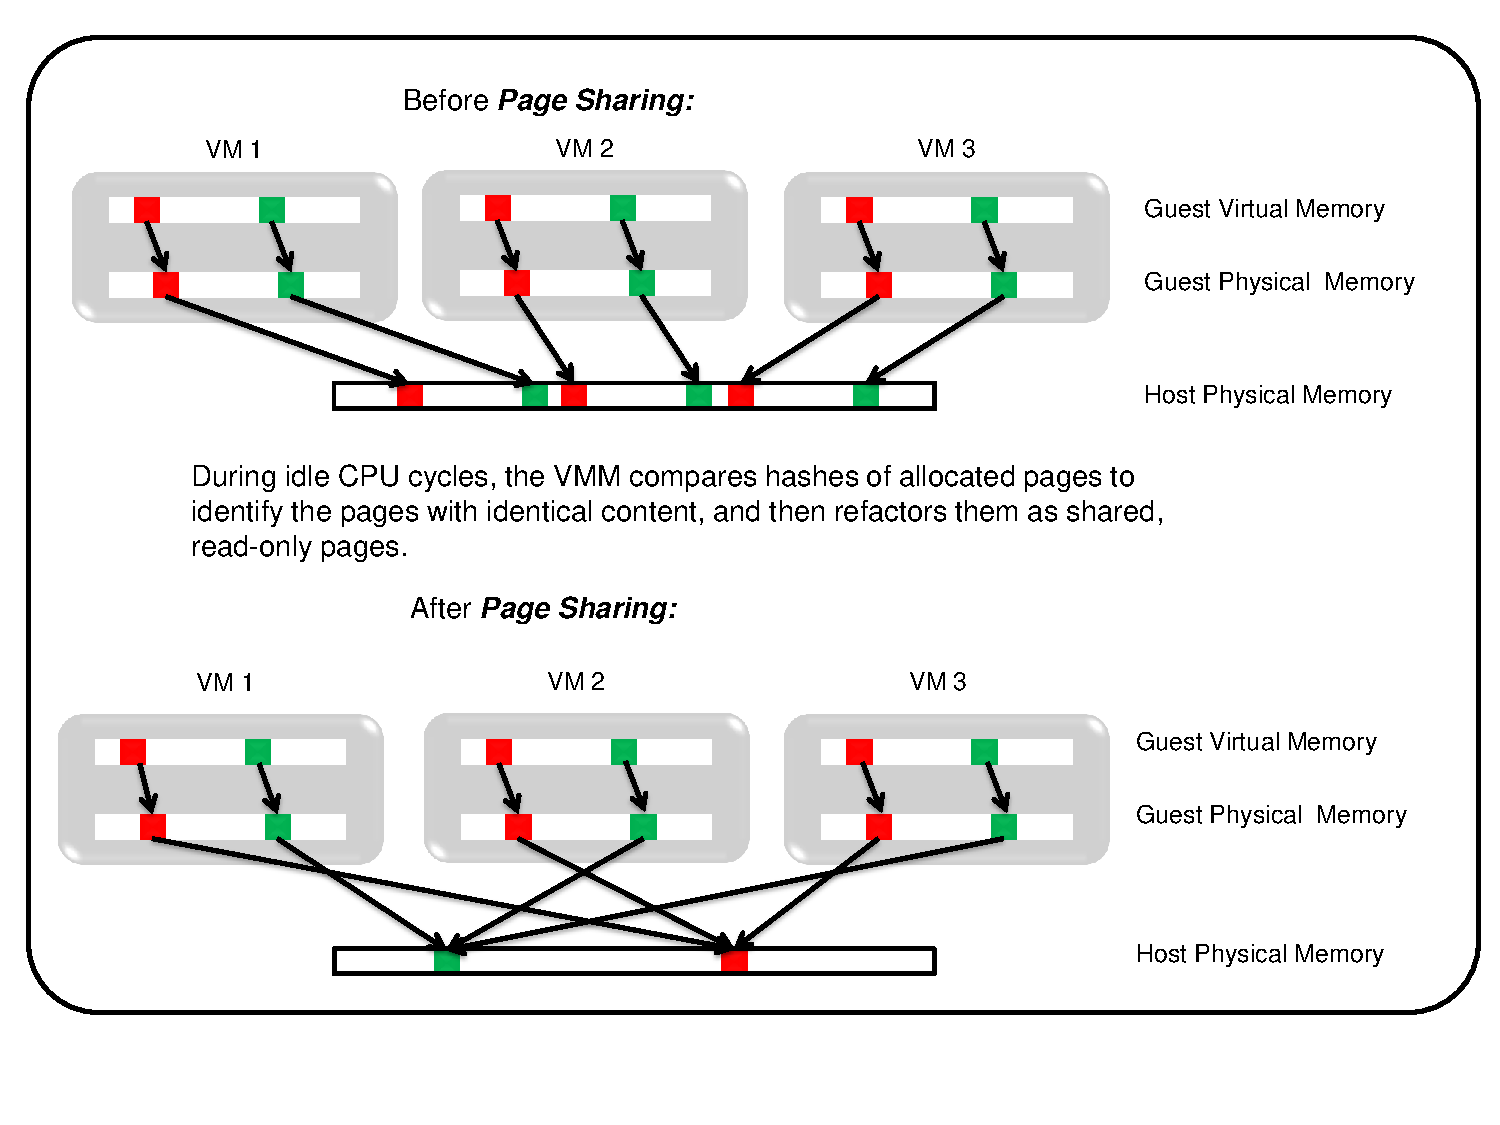
\includegraphics[scale=0.55, trim=1cm 0cm 2cm 0cm]{pagesharing.pdf}  
  \caption[{\em Transparent Page Sharing}]%
          {{\em Transparent Page Sharing}}
          \label{pagesharing}
  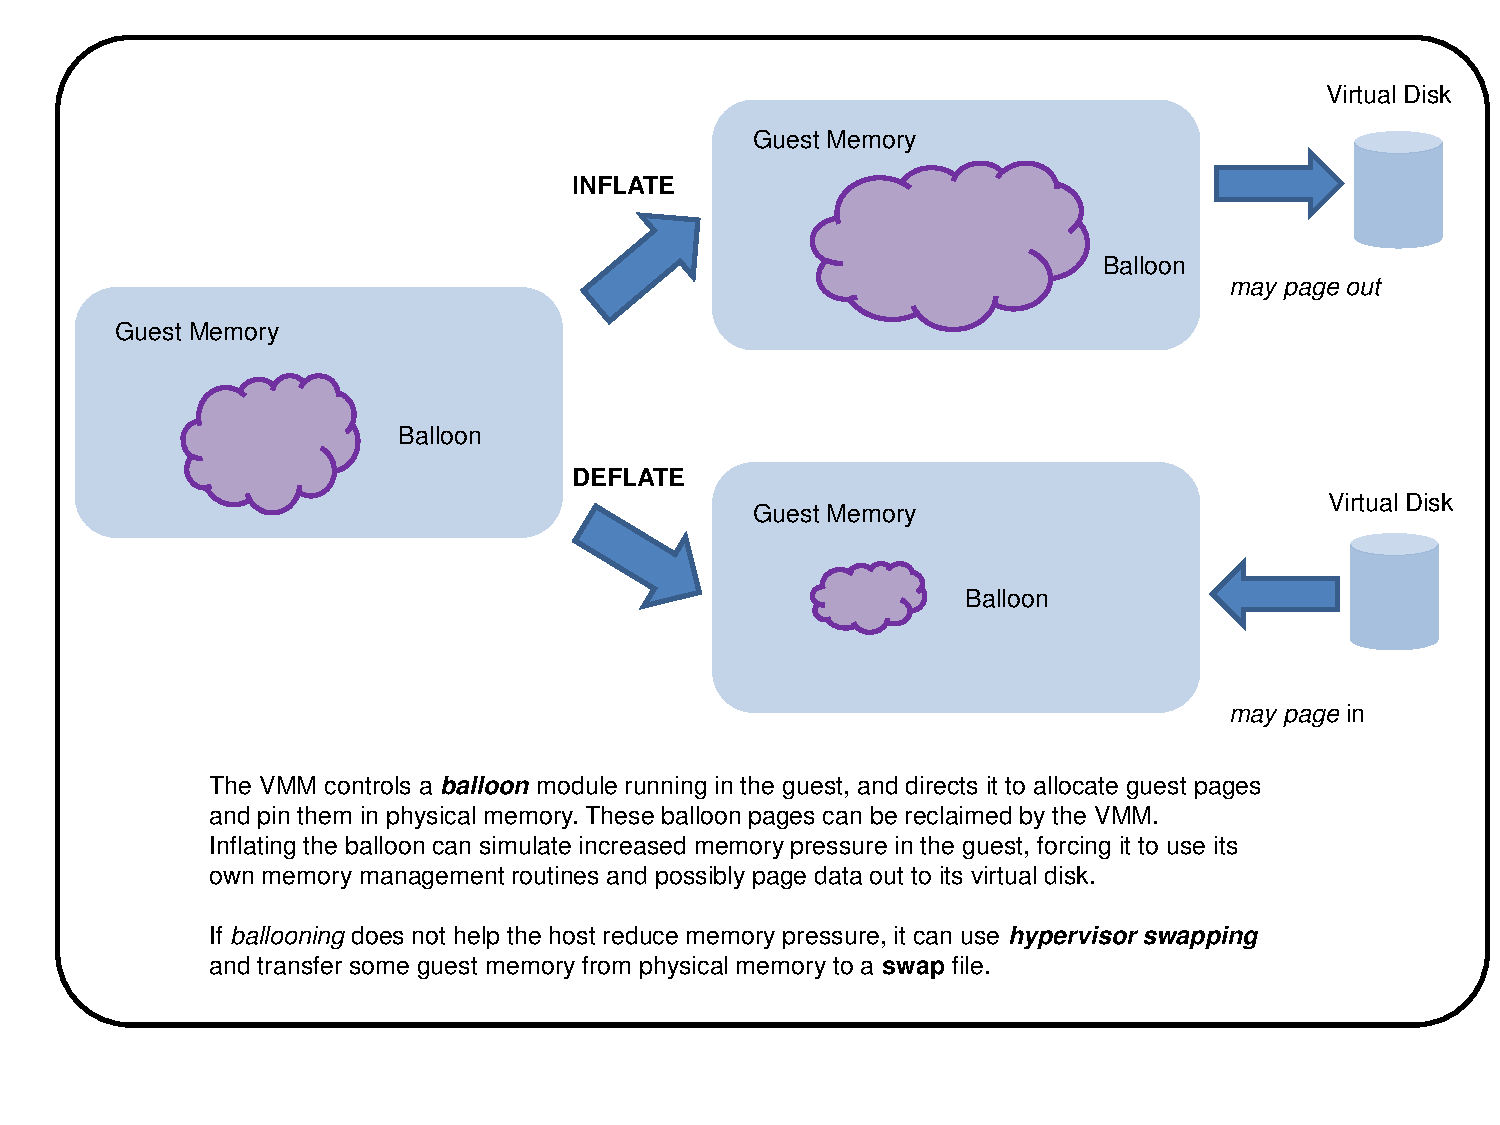
\includegraphics[scale=0.58, trim=1cm 0cm 1cm 0cm]{balloon.pdf}   
  \caption[{\em Ballooning} and {\em Hypervisor Swapping}]%
          {{\em Ballooning} and {\em Hypervisor Swapping}}
          \label{balloon}
\end{figure}

The ability to consolidate many VMs
on the same physical host is so important to the success
of server virtualization that many companies 
aggressively try to increase {\em VM density per host},
even in production environments.
For instance, {\em transparent page sharing}, {\em ballooning}
and {\em hypervisor swapping} (Figures \ref{pagesharing} and \ref{balloon})
allow a host to run many VMs with
combined memory requirements
that {\em exceed} the total physical memory
available on the host machine \cite{waldspurger2002memory}.

Apart from improvements in virtualization technology, two trends 
are expected to contribute to continually increase
VM density per host in the future:
newer generations of processors are expected to support more cores and 
memory \cite{hansen2010lithium} and the use of virtualization technology
for desktop machines \cite{vmwarevdi} in data centers.


In a Virtual Desktop Infrastructure \cite{vmwarevdi} (VDI), 
desktop operating systems and applications are hosted in 
virtual machines that reside in a data center; 
users access virtual desktops from desktop PCs or thin clients
via a remote display protocol. A VDI provides simplicity 
in administration and management: applications
can be centrally added, deleted, upgraded and patched. 
VDI deployments also promise even
higher consolidation ratios than those achieved via server virtualization
because desktop virtual machines typically require
less resources than server virtual machines.

Consolidation ratios (measured by VM density per host) in data centers



However, correlated spikes in the CPU/memory usage of many VMs can suddenly 
cripple host machines. For instance, a \emph{boot storm} \cite{hansen2010lithium, 
liao2011vmstore, meng2010tide, rajan2010vdc, vaghani2010virtual}
can occur after some software is installed or updated, requiring hundreds 
or thousands of identical VMs to reboot at the same time.
Bootstorms can be particularly frequent in VDIs because 
users typically show up to work at roughly the same time
in the morning each day. 

Concurrently booting VMs create unusually high I/O traffic,
generate numerous disk and memory allocation requests,
and can saturate host CPUs. 
To avoid the prohibitively high boot latencies that  
result from boot storms, data centers usually either 
boot machines in a staggered fashion, or invest in specialized,
expensive and/or extra-provisioned hardware for network/storage \cite{highperfnas, liao2011vmstore}.
There is also anecdotal evidence that VDI users sometimes leave their desktop computers running
overnight to avoid morning boot storms; this practice
represents an unnecessary addition to already exorbitant
data center energy bills \cite{qureshi2009bills}. Data deduplication \cite{clements2009deduplication},
through which hosts reclaim/reuse disk blocks common to several VMs, 
has been proven to reduce the memory footprint of concurrently
booting machines. However, while data deduplication can mitigate the stress on the memory subsystem in
a boot storm, lowered memory latency can in turn overwhelm the CPU, 
fibre channel, bus infrastructure or controller resources 
and simply turn them into bottlenecks instead \cite{netappstorm}. 

With the spread of virtualization, it is important to address the
bootstorm problem in a way that does not involve simply skirting around the
issue. Data deduplication is partly effective because identical VMs load
the same data from disk when they boot up. In this thesis, we pose the following question: 
is it possible to generalize deduplication of data to deduplication of \emph{execution}?
If many identical VMs are concurrently booting up in a data center, 
do they execute the same set of instructions? Even if there are
some differences in the instructions executed, are they caused by
controllable sources of non-determinism? Ultimately, if there is a way
to ensure that concurrently booting VMs execute mostly the same set of instructions
and perform the same I/O requests, one way to solve the boot storm
problem may be remarkable simple in essence: instead of booting
$N$ identical VMs concurrently, we can boot one VM as a leader; the remaining $(N-1)$ VMs 
follow the leader by executing a tiny subset of the instructions they would otherwise execute;
we split execution into $N$ different instances as late as possible into the boot process. This approach
could potentially reduce pressure on the underlying host hardware,
and thereby enable data centers to handle boot storms effectively.

\section{Goal of Thesis}
This thesis aims to address the following questions:

\begin{enumerate}

\item When identical VMs boot up concurrently, how similar
are the sets of instructions executed? What is the statistical
profile of any differences in the executed instructions?

\item What are the source(s) of any differences in
the instruction streams of concurrently booting VMs?
Are there ways to minimize the non-determinism in
booting VMs?

\end{enumerate}

The answers to these questions are clearly crucial in determining
the feasibility of \emph{deduplication of execution} as a possible solution
to the boot storm problem. 

\section{Contributions}
For this work, we used dynamic instrumentation frameworks such as
DynamoRio \cite{bruening2004dr} and Pin \cite{luk2005pin}
to study user-level instruction streams from 
a few representative Linux services at boot-time. \newline

In this document, we:
\begin {enumerate}
\item quantify nondeterminism in Linux services, and show that it is
  bursty and rare;
\item document the sources of nondeterminism in Linux services -- both obvious and obscure --
  and specify strategies for overcoming them in the boot storm scenario;
\item use simple dynamic instrumentation techniques to show that \emph{fully} deterministic execution is achievable
  without \emph{any} modifications to Linux or an executing service.
\end {enumerate}

Strategies to achieve deterministic execution have been studied at the operating system layer \cite{bergan2010dos} before,
but they require modifications to Linux. Deterministic execution can be achieved in multi-threaded programs 
using record-and-replay approaches \cite{patil2010pinplay} or deterministic logical clocks \cite{marek2011scaling}. 
Our study of non-determinism has different goals from from both approaches: we wish to avoid changing existing 
software (to ease adoption); we also wish to make several distinct -- and potentially different -- executions \emph{overlap} as much as possible, 
rather than replay one execution over and over. In our case, we do not know \emph{a priori} whether two executions 
will behave identically or not. That the behavior of system calls or signals in Linux can lead to different results or side-effects across
multiple executions of an application is well known: what is not documented is the application \emph{context} in
which these sources of nondeterminism originate. To the best of our knowledge, this is
the first attempt to study the statistical profile and context of nondeterminism in Linux services
in such detail. While we we hope
this work ultimately proves the basis for an implementation of our proposed solution to the boot storm
problem, we also note that deterministic execution can immediately improve
the effectiveness of existing virtualization technologies such as transparent page sharing
and data deduplication.

\section{Importance of Deterministic Execution}
While our study of nondeterminism is driven by a specfic application,
deterministic execution is desirable in a variety of scenarios.
%Our work complements existing
%work because it focuses on deterministic execution of primarily single-threaded services in Linux,
%at the granularity of individual instructions and their side-effects in
%memory.
The motivations for deterministic multhreading listed in
\cite{marek2011scaling, patil2010pinplay} apply to our work as well. \newline

\noindent {\bf Mainstream Computing, Security and Performance:}
If distinct executions of the same program can be
expected to execute the same set of instructions, then
any significant deviations can be used to detect security
attacks. Runtime detection of security attacks through the
identification of anomalous executions is the focus of \emph{mainstream computing} \cite{stephenson2010mainstream},
and deterministic execution obviously helps in reducing false
positives. 
Anomalous executions can also be flagged for performance
debugging. \newline

\noindent {\bf Testing:} 
Deterministic execution in general facilitates testing,
because outputs and internal state can be checked at 
certain points with respect to expected values. Our version
of determinism allows for a particularly strong kind
of test case that may be necessary for safety-critical 
systems: a program 
must execute the exact same instructions 
across different executions (for the same inputs). \newline 

\noindent {\bf Debugging:} 
Erroneous behavior can be more easily reproduced
via determininstic execution, which
helps with debugging. Deterministic
execution has much lower storage overhead
than traditional record-and-replay approaches. 

\section{Thesis Organization} 
In what follows, Chapter \ref{ch:boot} presents an overview of
the Linux boot process, along with the dynamic instrumentation
techniques we used to profile non-determinism in Linux services.
Chapter \ref{ch:src} presents a summary of the sources of nondeterminism
discovered in this work and the strategies we used
to eliminate them. 
Chapter \ref{ch:case} presents a detailed case study of three Linux services
to identify the common context in which non-determinism arises.
Chapter \ref{ch:design} presents design ideas for an implementation of deduplication of execution.
Finally, Chapter \ref{ch:conc} concludes this thesis and discusses future work.
